\documentclass[border=10pt]{standalone}
\usepackage{tikz}\usepackage{amsmath}\usetikzlibrary{arrows.meta}
\begin{document}
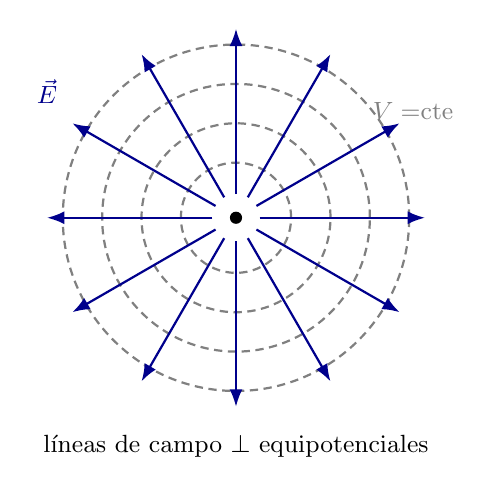
\begin{tikzpicture}[line width=0.8pt,>={Latex[length=2.2mm]}]
  \fill (0,0) circle(2.2pt);
  % equipotenciales: circulos discontinuos
  \foreach \r in {0.7,1.2,1.7,2.2} \draw[densely dashed,gray] (0,0) circle(\r);
  % lineas de campo: radiales solidas
  \foreach \a in {0,30,...,330} \draw[->,blue!55!black] (\a:0.3)--(\a:2.4);
  \node[gray] at (2.25,1.35){\small $V=$cte};
  \node[blue!55!black] at (-2.4,1.6){\small $\vec E$};
  \node at (0,-2.9){\small líneas de campo $\perp$ equipotenciales};
\end{tikzpicture}
\end{document}
